\documentclass[10pt,letterpaper]{article}
\usepackage[margin=.82in]{geometry}
\usepackage[T1]{fontenc}\usepackage{lmodern,graphicx,booktabs,amsmath,xcolor,hyperref,xurl,caption,fancyhdr}
\hypersetup{colorlinks=true,urlcolor=teal,linkcolor=teal,pdftitle={Check the denominator before claiming broadband coverage gains},pdfauthor={James Jean}}
\pagestyle{fancy}\fancyhf{}\fancyhead[L]{\small Broadband map denominators / Study 35}\fancyhead[R]{\small Independent descriptive audit}\fancyfoot[C]{\thepage}
\setlength{\headheight}{14pt}\setlength{\parindent}{0pt}\setlength{\parskip}{6pt}\captionsetup{font=small,labelfont=bf,hypcap=false}
\begin{document}
{\small\color{teal} PUBLIC AVAILABILITY DATA / MEASUREMENT BEFORE ATTRIBUTION\par}
\vspace{7pt}{\LARGE\bfseries Check the denominator before\par claiming broadband coverage gains\par}
\vspace{7pt}James Jean \hfill 30 October 2026

\textbf{Decision.} A larger reported broadband availability percentage does not by itself count new connections. The share depends on both the implied number of units reported served and the units included in the map. Preserve that denominator and the source version before interpreting a change as investment progress.

\textbf{Measured finding.} At the 100/20 Mbps source speed definition, a positive arithmetic denominator component accompanies 20 of 90 later state transitions with reported share gains. Across all 102 state transitions at that speed, the mean denominator component is -0.399 percentage points, while the mean reported change is 0.750 points. Denominator movement can therefore work in either direction. These are equal-geography descriptive comparisons, not causal effects or counts of new service.

\begin{center}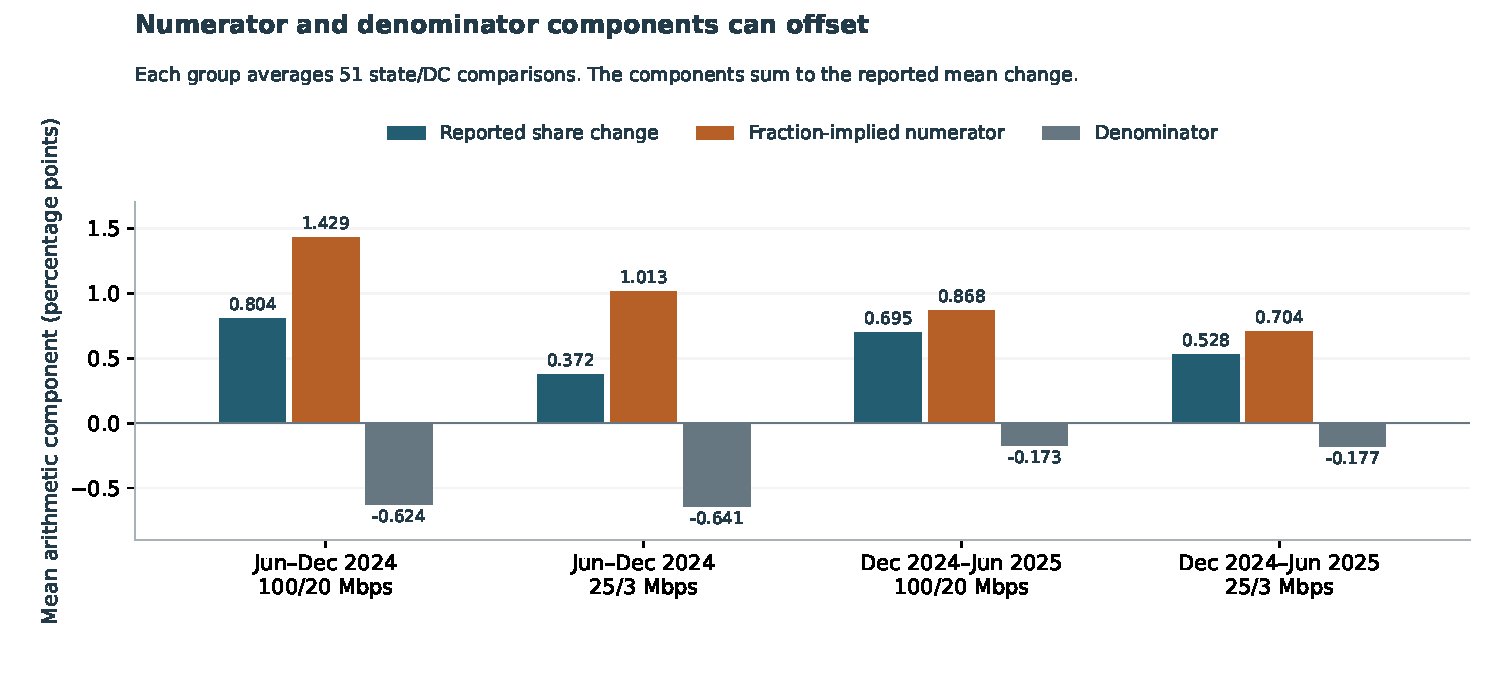
\includegraphics[width=\linewidth]{images/offsetting_components.pdf}\end{center}
\captionof{figure}{The fixed symmetric accounting convention separates fraction-implied numerator and denominator components. They sum to the reported share change before display rounding. Groups average the same state/DC cohort; speed rows share inputs and are not independent observations. Neither component identifies physical construction, source corrections or adoption. Source: FCC Broadband Data Collection; processed by this study.}

\textbf{Practical recommendation.} Retain native geographic/service keys, total units, source shares, data dates and revision dates. Show signed components and an infeasibility reason rather than calling all share growth new coverage. Location-level lineage, provider corrections and independent delivery evidence are still needed before attributing a change to construction or measured public benefit.
\newpage
\section*{1. A complete, bounded public-summary cohort}
Four exact public FCC aggregate ZIPs yield 204 eligible source rows across 51 states/DC and 4 data dates, with 408 native speed-share cells plus an integer unit denominator per row. The reader scans 2,487,660 original aggregate records. All fixed keys are present, without duplicate copies or conflicting values. The original ZIPs and CSV members remain privately preserved with hashes and CRC checks; only the minimal attributed projection and new calculations are public.
\begin{center}\small\begin{tabular}{@{}llr@{}}\toprule
Data as-of date & Native filename revision date & State/DC keys\\\midrule
2023-12-31 & 2025-12-24 & 51 \\
2024-06-30 & 2026-07-27 & 51 \\
2024-12-31 & 2026-07-29 & 51 \\
2025-06-30 & 2026-10-01 & 51 \\
\bottomrule\end{tabular}\end{center}

\textbf{Meaning before arithmetic.} The fixed source stratum is State / Total / R / Any Terrestrial, with 25/3 and 100/20 Mbps source speed fields. The specification uses the label \textit{All Terrestrial}; the CSV literal is \textit{Any Terrestrial}. That explicit binding was committed before comparisons. No satellite-inclusive alternative, overlapping provider total or sum of technology rows is substituted. R is retained as the publisher's native coded stratum; this study does not reconstruct every underlying mixed-use classification rule.

The specification defines total\_units as the sum of units in broadband serviceable locations in the geography. These are aggregate map units, not subscribing households, people or a list of individual buildings. A location can contain multiple units. The source shares describe reported availability at maximum advertised speed tiers, not adoption, affordability, measured delivered speed or customers connected. All nine native decimal places are retained, although the specification's examples use four.

\begin{center}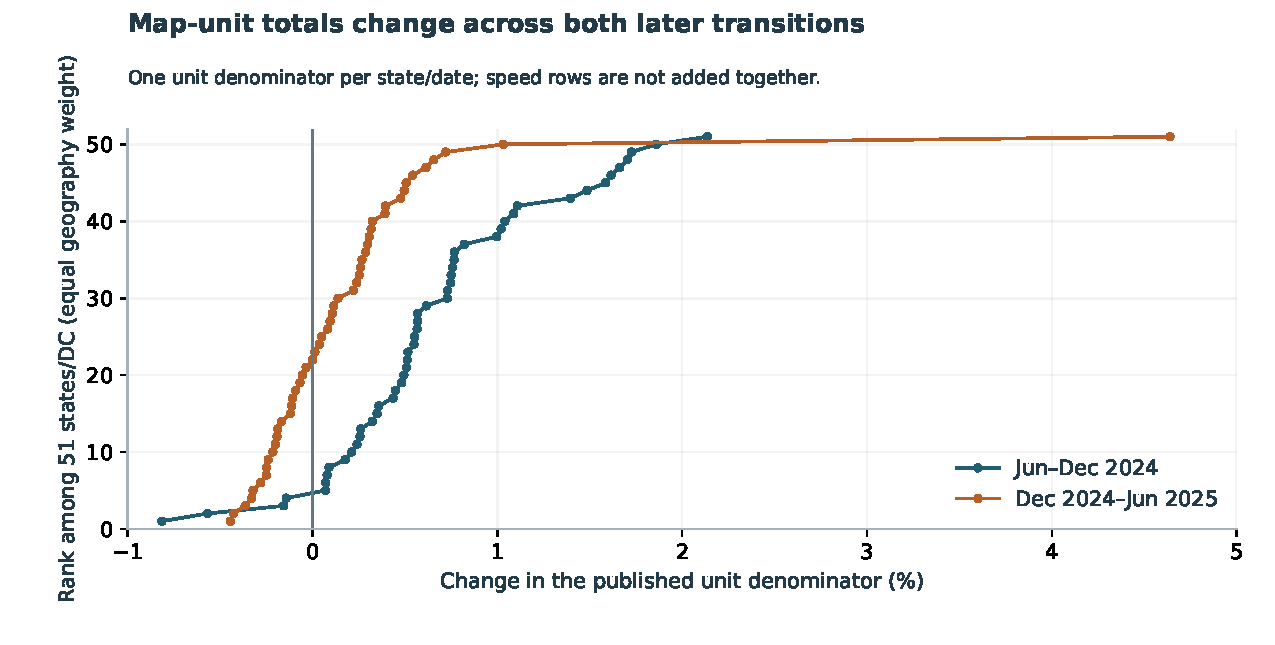
\includegraphics[width=.94\linewidth]{images/unit_denominator_changes.pdf}\end{center}
\captionof{figure}{Every later state/DC denominator change is retained once per transition. Unit totals are shared by the two speed fields and are not added twice. Ranks use equal geography weight, not population weights. Changes can reflect underlying data, classification, model updates or other mechanisms; aggregate differences alone do not identify a reason. Retrieved revision dates are not certified original publication vintages.}
\newpage
\section*{2. Exact accounting and a declared counterfactual}
For adjacent source dates, let $N_0,N_1$ be published map-unit totals and $p_0,p_1$ the published fractions. Define $I_0=N_0p_0$ and $I_1=N_1p_1$. These are \textbf{fraction-implied quantities}, not exact observed integer counts of served units. The descriptive share change is $\Delta=100(p_1-p_0)$ percentage points.
\begin{align*}
S&=50(I_1-I_0)(1/N_0+1/N_1),\\
D&=50(I_0+I_1)(1/N_1-1/N_0),\\
S+D&=\Delta.
\end{align*}
$S$ is the fraction-implied numerator component and $D$ the denominator component. This convention averages the two orders of substituting numerator and denominator; 50 is 100 times the one-half order weight. It was fixed before values and is not fitted to improve an outcome. The identity is elementary arithmetic, not a newly discovered causal relationship.

A second, explicitly authored diagnostic holds the baseline implied quantity fixed: $p_{\rm cf}=I_0/N_1$. Report its change from $p_0$ only if $I_0\le N_1$. Otherwise the counterfactual is infeasible and remains unavailable; it is not clipped to 100\%. A no-construction interpretation is not established by that calculation.

\textbf{Separation.} Development uses only December 2023 to June 2024: 102 state/speed pairs and 408 authored sensitivity endpoint cases. The earlier results below were independently checked before committing 32 dependency hashes, including source definitions, projection, code, checks, fixtures, exercise and exports. No model, threshold or preferred comparator is selected.
\begin{center}\small\begin{tabular}{@{}llrrrrr@{}}\toprule
Transition & Mbps & Pairs & Mean$\Delta$ & Mean$S$ & Mean$D$ & $D>0$\\\midrule
Dec23--Jun24 & 100/20 & 51 & 1.199 & 1.244 & -0.045 & 21 \\
Dec23--Jun24 & 25/3 & 51 & 0.733 & 0.781 & -0.047 & 21 \\
\bottomrule\end{tabular}\end{center}

\textbf{Sensitivity, not a confidence interval.} Independently perturb each source fraction by plus/minus 0.0001 and clip the proposed endpoints to [0,1]. Enumerate all four endpoint combinations with exact fractions, recompute $\Delta,S,D$, and retain minima/maxima and sign stability. This fixed 0.01-percentage-point perturbation was motivated by the specification's example precision before the nine-decimal source values were captured. It is an authored numerical sensitivity, not a native rounding bound, source-error guarantee, probability model or sampling interval.

Full source values were exposed for rights, schema and fixed-key qualification. Binding occurred after capture; no analyst-blindness or untouched-schema claim. Later comparisons were not generated before the committed dependency manifest.
\newpage
\section*{3. Later accounting, with both directions visible}
The later check retains 204 state/speed pairs across two adjacent transitions. Every native fact, exact component, counterfactual state and source key remains in the public observation exports. The means below use equal state/DC weight and are in percentage points.
\begin{center}\small\begin{tabular}{@{}llrrrrr@{}}\toprule
Transition & Mbps & Pairs & Mean$\Delta$ & Mean$S$ & Mean$D$ & $D>0$\\\midrule
Jun--Dec24 & 100/20 & 51 & 0.804 & 1.429 & -0.624 & 4 \\
Jun--Dec24 & 25/3 & 51 & 0.372 & 1.013 & -0.641 & 4 \\
Dec24--Jun25 & 100/20 & 51 & 0.695 & 0.868 & -0.173 & 21 \\
Dec24--Jun25 & 25/3 & 51 & 0.528 & 0.704 & -0.177 & 21 \\
\midrule
Pooled later & 100/20 & 102 & 0.750 & 1.148 & -0.399 & 25 \\
Pooled later & 25/3 & 102 & 0.450 & 0.859 & -0.409 & 25 \\
\bottomrule\end{tabular}\end{center}

\textbf{Interpretation.} The denominator component is negative on average at both source speed definitions. Positive denominator components accompany some reported improvements, but it would be wrong to describe every gain as an artefact. It would also be wrong to label the remaining numerator component construction: it inherits availability reporting, unit definitions, revisions and the precision of the source fraction. No cause is identified from the aggregate accounting alone.

\textbf{Worked later case: North Dakota, 100/20 Mbps.} From December 2024 to June 2025, a modest reported share increase combines much larger offsetting components. The published total-unit change is retained; the study does not infer why those map units changed.
\begin{center}\small\begin{tabular}{@{}lr@{}}\toprule
Quantity & Value\\\midrule
Baseline map units & 477,239 \\
Later map units & 499,377 \\
Baseline published share (\%) & 99.587628 \\
Later published share (\%) & 99.839200 \\
Reported change (pp) & 0.251572 \\
Fraction-implied numerator component (pp) & 4.774646 \\
Denominator component (pp) & -4.523075 \\
\bottomrule\end{tabular}\end{center}

Displayed values are rounded only for reading; native share tokens, exact rational products and identity residuals are retained. The source's fraction-implied numerator quantities need not be integers. A larger positive $S$ does not establish a corresponding number of new connected households, nor does a negative $D$ show that real-world service declined.

The state transitions share geographies, dates, provider reports and map inputs; the two speed definitions share unit denominators and nested availability concepts. The rows are descriptive repeated measurements, not independent trials. No p-value, population-weighted national estimate, deployment result, realized saving or causal investment effect is presented.
\newpage
\section*{4. Keep infeasibility and sensitivity visible}
At each speed, 101 later counterfactuals are feasible and 1 is infeasible. The latter is DC's December 2024 to June 2025 transition. Its baseline fraction-implied quantity exceeds the newer published total. Keeping that quantity fixed would produce a fraction greater than one, so the counterfactual returns unavailable instead of silently clipping it.

\begin{center}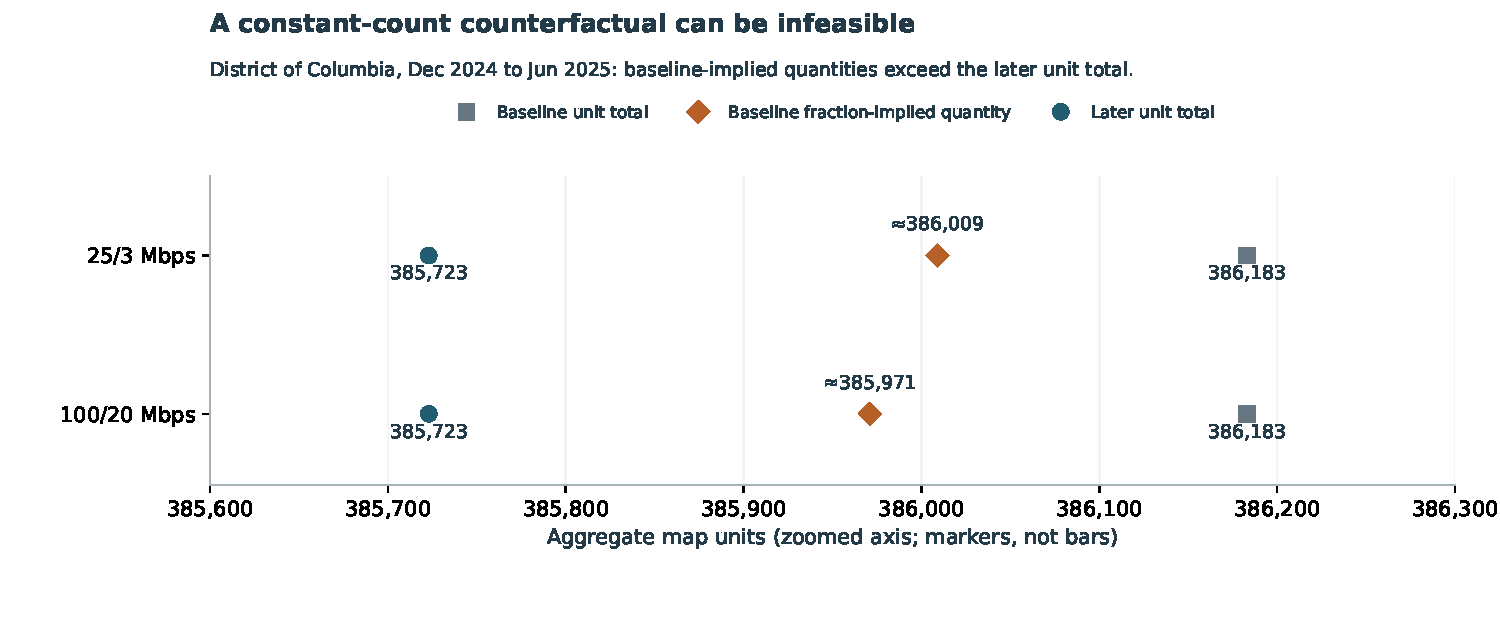
\includegraphics[width=\linewidth]{images/infeasible_counterfactual.pdf}\end{center}
\captionof{figure}{Both speed definitions for the retained infeasible transition. Markers use an explicitly zoomed unit axis; no bar length implies a zero baseline. Approximate labels identify fraction-implied quantities, while native total-unit counts remain exact. This identifies an inconsistent counterfactual assumption, not proof that the source data themselves are wrong.}

All 816 authored later sensitivity cases remain available. The table reports stable signs under the declared perturbation; zero is a separate exported state, with no zero-stable case in these rows. Ambiguity is not converted into a correct negative result.
\begin{center}\small\begin{tabular}{@{}llrrr@{}}\toprule
Mbps & Quantity & Stable positive & Stable negative & Ambiguous\\\midrule
100/20 & Reported change & 89 & 11 & 2 \\
100/20 & Numerator & 89 & 11 & 2 \\
100/20 & Denominator & 25 & 77 & 0 \\
25/3 & Reported change & 85 & 10 & 7 \\
25/3 & Numerator & 87 & 12 & 3 \\
25/3 & Denominator & 25 & 77 & 0 \\
\bottomrule\end{tabular}\end{center}

\textbf{Implementation exercise.} Authored examples produce the same 10-point share increase in two ways: 100 units at 0.9 moving to 90 units at 1 leaves the implied quantity unchanged, while 100 units at 0.9 moving to 100 units at 1 leaves the denominator unchanged. The reference CLI returns their different exact components and checks identity, dates, count/share units and counterfactual feasibility. These are invented examples, not FCC records or causal demonstrations. A matching input label cannot authenticate a source or recover licensed location lineage.
\newpage
\section*{5. Checks, limits and next evidence}
Independent DuckDB parsing, SQL and exact fractions reconcile 2,892 original-row/token conditions. The main standard-library reader and independent source parser retain exact strings and do not rewrite source archives. Independent source joins and two-order arithmetic pass 6,395 development conditions and 12,023 later conditions. The 42 finite fixtures cover missing/conflicting keys, source categories, units and scale, nesting, exact cancellation, unchanged inputs, infeasible counterfactuals, clipped endpoints and the offline input guard.

The public numerical replay validates the committed freeze in a full-history local clone, regenerates outputs into separate paths, compares exact CSV fields and JSON content, and preserves frozen bytes. Original-source reconciliation is an additional optional check requiring the captured ZIPs; recapturing an old data date does not prove identical historical bytes. Figure checks bind source queries to actual SVG coordinates and export hashes. The manuscript retains a numerical display ledger, LaTeX and figure PDFs, with separate rendered-page inspection.

\textbf{Source and version limits.} These are aggregate R-coded terrestrial availability summaries. Native category names and the specification differ and are explicitly retained. The study does not reconstruct every mixed-use classification rule, individual Fabric record or underlying provider-level service claim. Total map units are not people, unique buildings, subscriptions or independently observed served counts. Data-as-of, filename-revision and visible UI-update dates remain separate. Retrieved historical summaries are not original first-release vintages.

\textbf{Scientific limits.} The symmetric decomposition and counterfactual are declared conventions. Exact arithmetic does not establish source truth or causal identification. The fixed sensitivity is not a confidence interval or error bound. Shared source inputs and repeated geographies preclude treating the finite rows as independent trials. No trained model, location-level spatial join, Census API analysis, new estimator, scientific-priority claim, realized public benefit or peer review is established. This independent program manuscript excludes separate formal-publication projects.

\textbf{Next evidence.} A planning team should preserve geographic/service keys and source-version lineage, inspect denominator changes, and retain unavailable results. To distinguish construction from corrections or changed map membership, obtain authorized matched location histories, provider revision/challenge records and independently verified delivery evidence. Use adoption and actual performance data for those separate questions. This aggregate diagnostic cannot replace that evidence.

\section*{Primary sources and reproducibility}
\small
[1] FCC, \href{https://broadbandmap.fcc.gov/data-download}{National Broadband Map public downloads}. Fixed Broadband Summary by Geography Type, four named data dates. Exact archive/member hashes, native revision dates, selected UI evidence and complete exclusions are retained.

[2] FCC, \href{https://us-fcc.app.box.com/v/bdc-data-downloads-output}{Specifications for Data Downloads from the National Broadband Map}, August 11, 2026, sections 2 and 3.1.3.5.1. Privately retained exact PDF snapshot, linked from the official BDC Key Reference Documents page.

[3] FCC, \href{https://broadbandmap.fcc.gov/about?version=jun2026}{About the map: data definitions, license and attribution}; \href{https://help.bdc.fcc.gov/hc/en-us/articles/12382207389083-Changes-to-the-Fabric-between-Versions}{Changes to the Fabric between Versions}. Availability data are offered free; individual CostQuest Fabric rights are reserved. No licensed individual records are included or reconstructed.

Code, native projection, all components/sensitivity cases, figures and exercise: \url{https://github.com/S3R3Bii/broadband-map-denominators}.
\end{document}
